\documentclass[../main.tex]{subfiles}
\graphicspath{{\subfix{../images/}}}
\begin{document}

%%%%%%%%%%%%%%%%%%%%%%%%%%%%%%%%%%%%%%%%%%%%%%%%%%%%%%%%%%%%%%%%%%%%%%%%%%%%%%%%
\section{Multimeter Basics}
\index{Electronics!Multimeter}

Multimeter is an important device that allows to measure the resistance of a
resistor or a voltage on a power supply, allows to perform continuity test of a
circuit, to check the polarity of an LED and check its color and so on.

You can see an example of a multimeter on fig. \ref{fig:multimeter-example}.

\begin{figure}[ht]
  \centering
  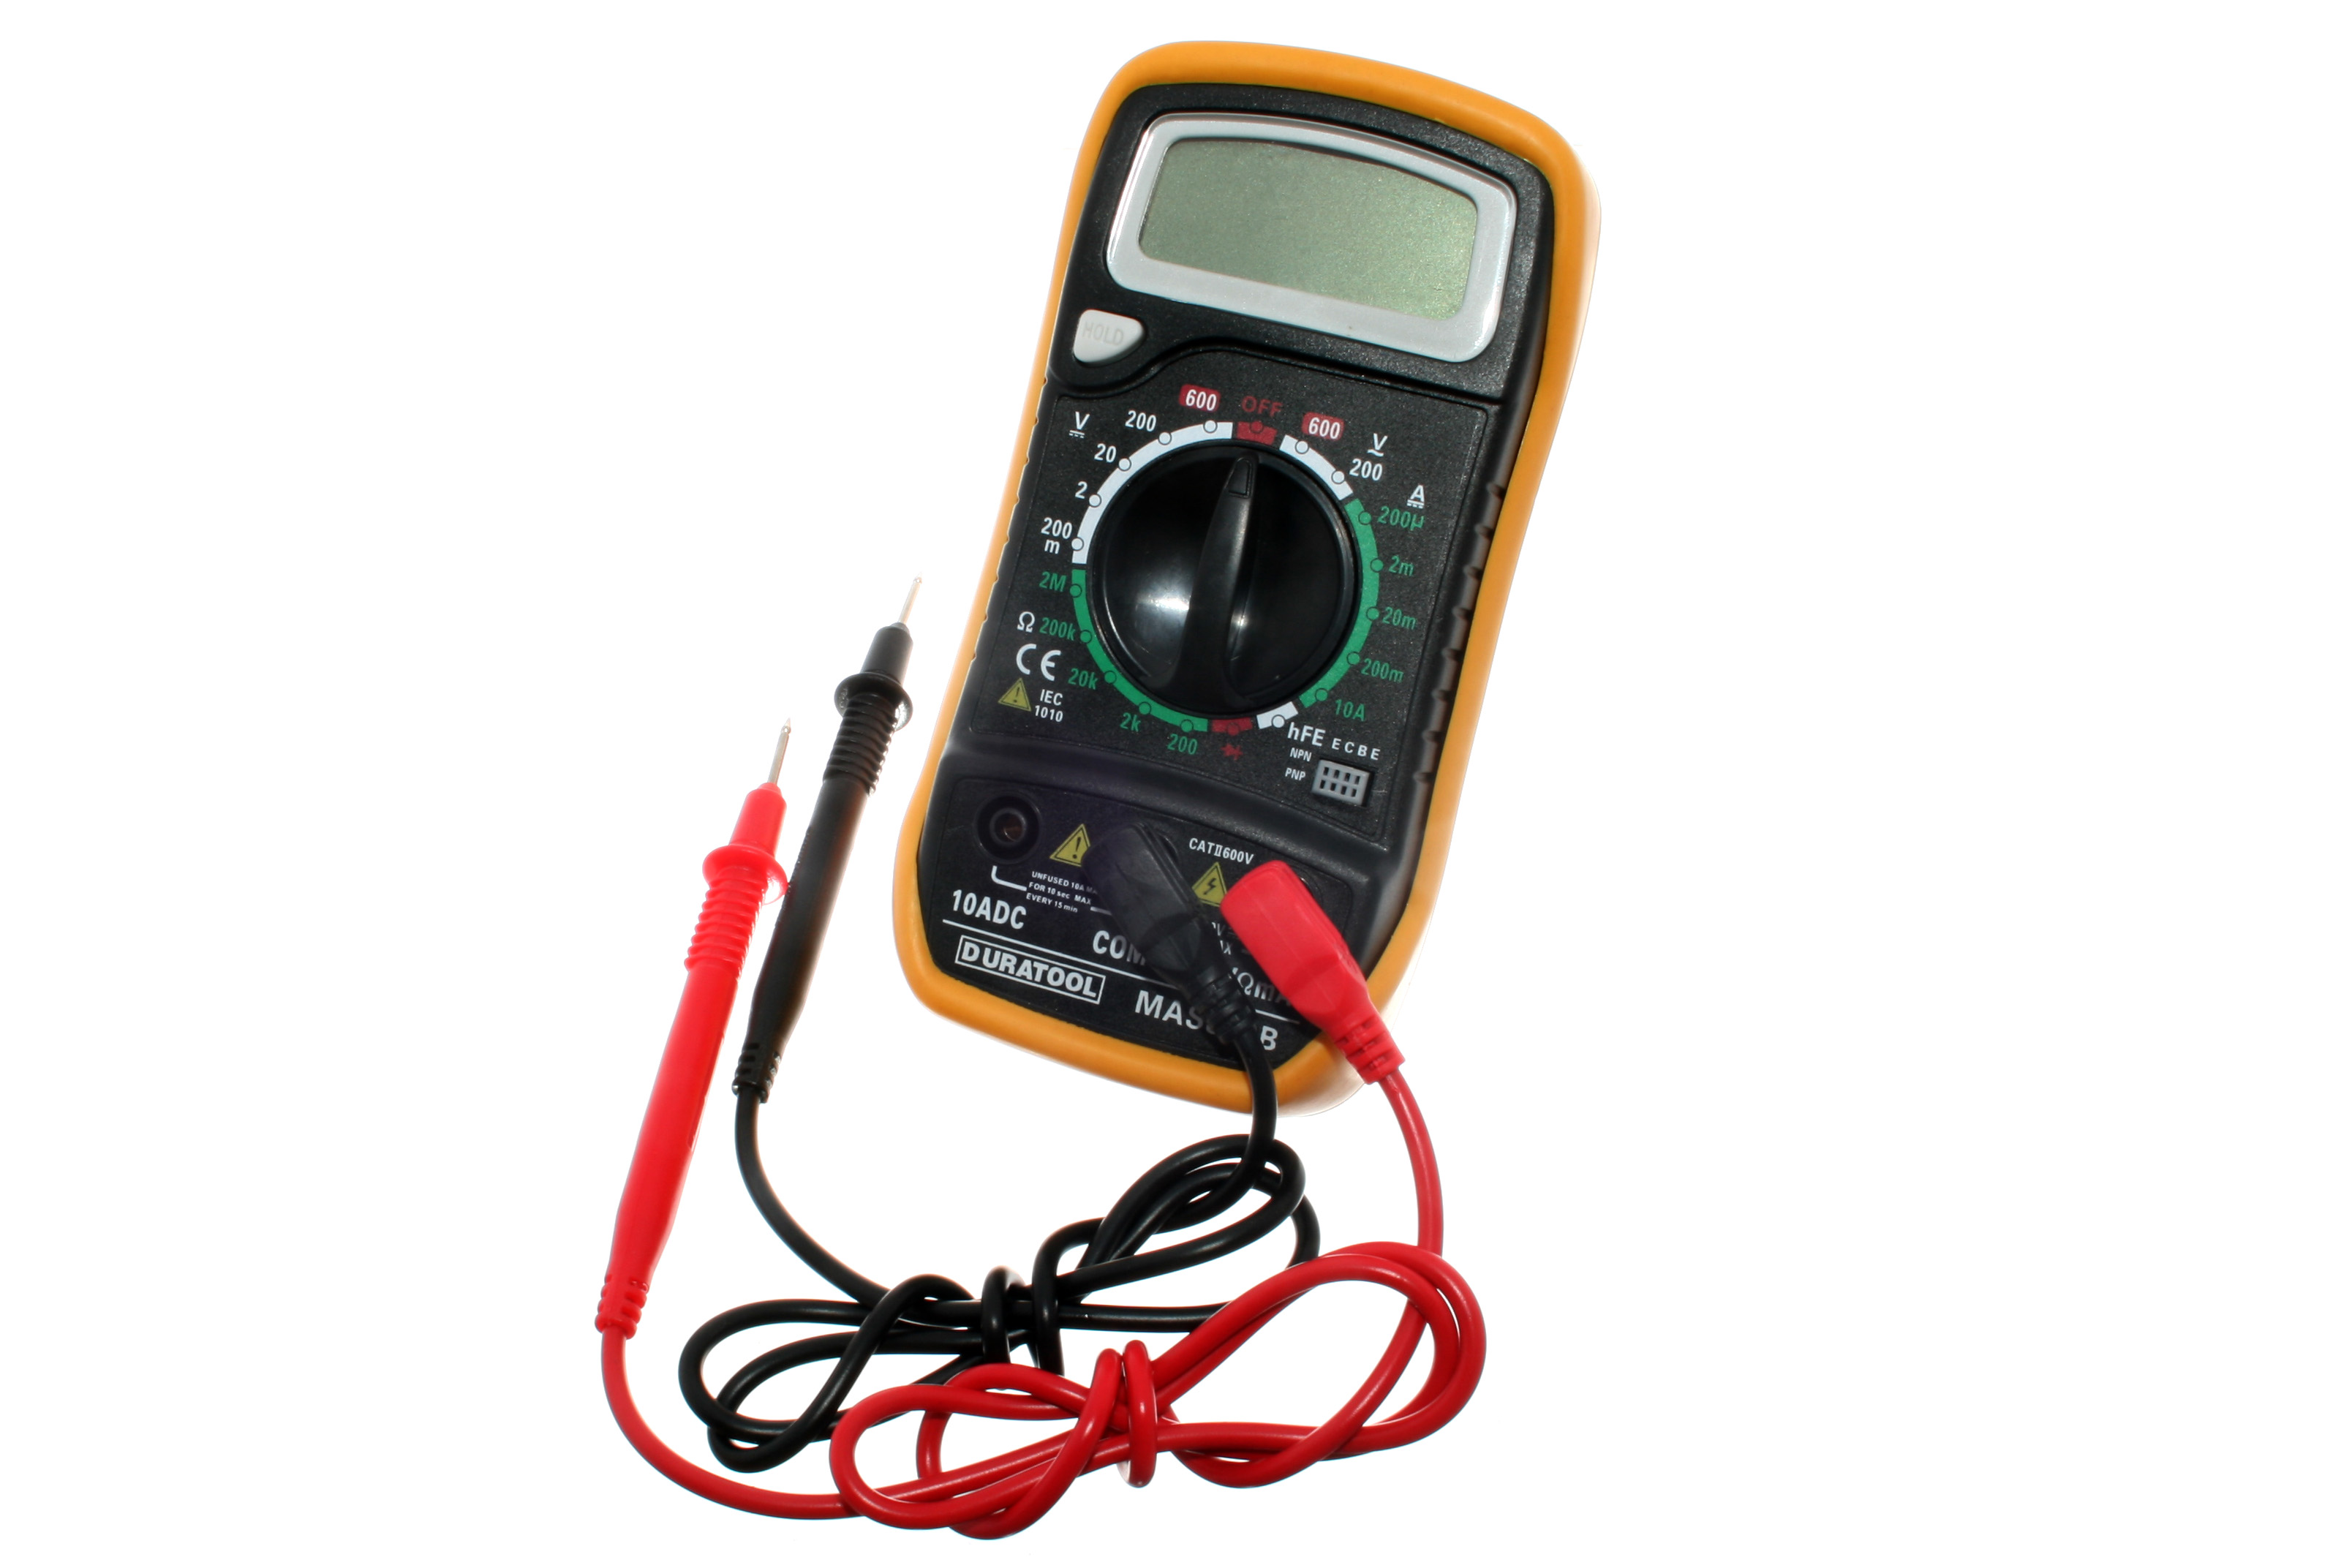
\includegraphics[width=14cm]{Digital_Multimeter}
  \caption{An example of a digital multimeter.}
  \label{fig:multimeter-example}
\end{figure}

%%%%%%%%%%%%%%%%%%%%%%%%%%%%%%%%%%%%%%%%%%%%%%%%%%%%%%%%%%%%%%%%%%%%%%%%%%%%%%%%
\subsection{Main Parameters of a Multimeter}

A multimeter measures current (instant) parameter values of electronic
components or circuits.  Depending on the multimeter model the speed of
``reaction'' on parameter value changes can vary but usually this multimeter
parameter is not important.

Overall, multimeters have four\cite{fluke:multimeter} main parameters:
\begin{itemize}
\item \textbf{Accuracy} refers to largest allowable error that occurs under
  specific operating conditions.
\item \textbf{Precision} refers to a multimeter's ability to provide the same
  measurement repeatedly.
\item \textbf{Resolution} refers to the smallest increment that a multimeter can
  detect and display.
\item \textbf{Range} refers to the lower and upper limits of measurements.
\end{itemize}

Let's discuss each of the parameters in details.

\emph{Accuracy} of a multimeter reflect the higher error value that can occur in
specific operating conditions during device exploitation.  This parameter is set
in percentage and shows how close is the resulting value of measurement to the
factual (standard) value of the measured signal.  This parameter is set in
percentage and the lower its value -- the better.

\emph{Precision} refers to the ability of a multimeter to reproduce each time
the measurements that are close to each other.  While a device with bad
\emph{accuracy} will produce measurements that are differ from the actual
values, when the \emph{precision} is good the scatter of readings will be
minimal.

When a device has good \emph{accuracy} and high \emph{precision} it produces
measurements that are not only close to the actual measured values but the
results will have very little scatter in repeated measurements of the same
value.

\emph{Resolution} of a multimeter sets the smaller step that the device can use
to make measurements.  Let's suppose that we're trying to measure the voltage on
a standard 1.5V battery.  If a digital multimeter has the resolution of 1mV in a
range of 3V then we will be able to see the change in 1mV during the
measurement.  Thus a user will be able to see a change in one-thousandth of a
Volt or 0.001V in a range of 3V.

The \emph{range} parameter is often linked to the resolution and sometimes is
described in the device specification.  Most of the multimeters have auto-range
functionality that allows to set the proper range of measurement automatically.
If the range is less than the measured value then digital multimeters usually
indicate an overload in some way.  The most precise measurements are done in the
smaller range of values that is sufficient to measure a signal without the
overload.

%%%%%%%%%%%%%%%%%%%%%%%%%%%%%%%%%%%%%%%%%%%%%%%%%%%%%%%%%%%%%%%%%%%%%%%%%%%%%%%%
\subsection{Conventional Designations on a Multimeter}

Here you can find a table that shows the main symbols that you can find on the
multimeter:

\begin{tabular}{| m{8em} | m{22em} |}
  \hline
  \textbf{Designation} & \textbf{Description} \\
  \hline
  V$\sim$ & Measurement of the voltage of alternating current (AC.) \\
  \hline
  mV$\sim$ & Measurement of the voltage of alternating current in the millivolts
  (mV) range. \\
  \hline
  V\textdirectcurrent{} & Measurement of the voltage of of the direct current. \\
  \hline
  mV & Measurement of the voltage of the direct current in millivolts (mV) range. \\
  \hline
  A\textdirectcurrent{} & Measurement of direct current. \\
  \hline
  A$\sim$ & Measurement of alternating current. \\
  \hline
  $\Omega$ & Measurement of the resistance.  Usually multimeters provide the
  following ranges: ``2k'' (2000 Ohms), ``20k'' (20'000 Ohms), ``200k'' (200'000
  Ohms) and ``2M'' (two mega-Ohms or 2'000'000 Ohms.)\\
  \hline
  HOLD & ``Freeze'' the current value on the display. \\
  \hline
  \esymbol{diode} & Diode continuity test. \\
  \hline
  Hz   & ``Hertz'' -- measurement of frequency. \\
  \hline
  \esymbol{capacitor} & Measurement of capacitance. \\
  \hline
  \soundWaveIcon{} & Circuit continuity test. \\
  \hline
  hFE & ``\textbf{H}ybrid parameter \textbf{f}orward current gain, common
  \textbf{e}mitter'' -- a mode for testing transistors. \\
  \hline
\end{tabular}

\end{document}
